\section{Local Outlier Factor}
\label{sec:LocalOutlierFactor}


The Local Outlier Factor (\gls{lof}) algorithm is effective in identifying outliers by assessing the density of instances surrounding a particular data point in comparison to the density around its neighbouring points. Typically, an anomaly is considered more isolated than its k nearest neighbours \citepage{hands-on-geron2022}{293}. 

Formally, the authors that designed this algorithm define the \gls{lof} of an instance $\gls{sym:snap}$ as the average of the ratio of the local reachability density of $\gls{sym:snap}$ and the local reachability density of its $MinPts$ k-nearest neighbours \cite{breunig2000lof}. This is a measure of how isolated the instance is with respect to the surrounding neighbourhood. 

Using this approach, this algorithm is able to identify outliers in a dataset with arbitrary shapes. Moreover, it can identify outliers in a dataset with different densities, as a point very near to a very dense \gls{glo:clust} can be declared as an outlier, while a point even more distant from a less dense \gls{glo:clust} could be declared as normal.

\subsection{Training}
\label{sec:lof_train}
\begin{figure}
    \centering
    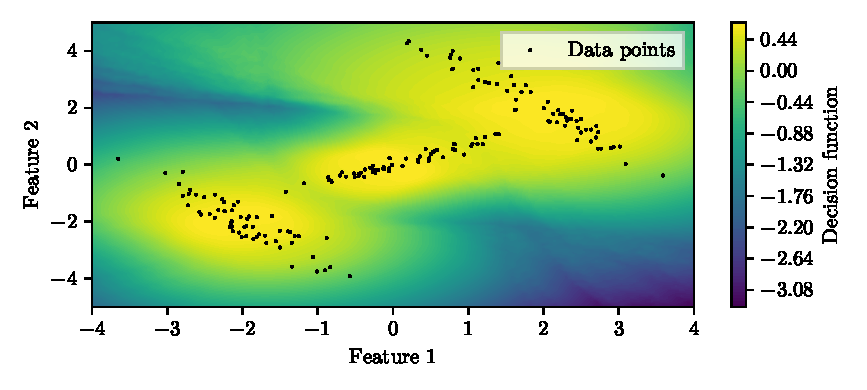
\includegraphics{images/LOF/Figure_1.pdf}
    \caption{Local Outlier Factor decision function.}
    \label{fig:LocalOutlierFactor}
\end{figure}
This algorithm is implemented in \texttt{sklearn} library and requires the number $MinPts$ of k-nearest neighbours to be specified. According to the authors, the value of \gls{lof} of a particular \gls{glo:snap} is neither increasing nor decreasing with the value of $MinPts$. They also suggest an \gls{glo:heuristic} to select the value of $MinPts$ that is hardly automatable. 
For this reason, it's difficult to use this algorithm in a real-time scenario in an unsupervised way.

Anyway, as an example, using the same dataset used in \autoref{fig:dbscandata}, and running the \gls{lof} algorithm with the default value of $MinPts=20$, we obtain the results shown in \autoref{fig:LocalOutlierFactor}.

\subsection{Evaluation of a new instance}
\label{sec:lof_eval}
The \texttt{sklearn} implementation of the \gls{lof} algorithm has a method that returns the \gls{lof} of a new instance. Since the bigger the value is, the more likely it is that the new \gls{glo:snap} is an outlier, we can take directly this value as a metric to evaluate the novelty of a new instance.

To select a threshold value, it holds what has been said in \autoref{sec:iforest_threshold} about \gls{iforest}.


\subsection{Limitations of Local Outlier Factor}
\label{sec:lof_limitations}
The main limitations are the difficulty of defining a threshold value to declare some instances as outliers and using this algorithm in a completely unsupervised way.


